\documentclass[12pt]{article}
\usepackage{fullpage,enumitem,amsmath,amssymb,graphicx}

\title{College Physics Homework 2 }
%\author{Deniz O. Devecioglu  -- \texttt{dodeve@hotmail.com}}

\begin{document}
  \maketitle,
  \begin{center}

  \vspace{-0.3in}
  \begin{tabular}{rl}
  Due: March 28 2022 & 
  \end{tabular}
  \end{center}
  This is an individual assignment; you must solve it by yourself.
  \noindent

  \rule{\linewidth}{0.4pt}
\section*{Problem 1}
\begin{enumerate}[label=(\roman*)]
\item Suppose that a uniform rope of length $L$, resting on a frictionless horizontal surface, is accelerated along the direction of its length by means of a force $F$ pulling it at one end. Derive an expression for the tension $T$ in the rope as a function of position along its length. How is the expression for $T$ changed if the rope is accelerated vertically in a constant gravitational field?
\item A mass $M$ is accelerated by the rope in part (i). Assuming the mass of the rope to be $m$, calculate the tension for the horizontal and vertical cases.
\end{enumerate}
\section*{Problem 2}
A particle sliding down a frictionless ramp is to attain a given \textit{horizontal} displacement $\Delta x$ in a minimum amount of time. What is the best angle for the ramp? What is the minimum time (give your answer in terms of $\Delta x, g$)?

\section*{Problem 3}
Two blocks of masses $m_{1}$ and $m_{2}$ are sliding down an inclined plane making an angle with the horizontal. The leading block ($m_{2}$) has a coefficient of kinetic friction $\mu_{k}$; the trailing block ($m_{1}$) has a coefficient of kinetic friction $2\mu_{k}$. A string connects the two blocks; this string makes an angle $\phi$ with the ramp (Fig. \ref{fig1}). Find the tension in the string.
\begin{figure}
\center
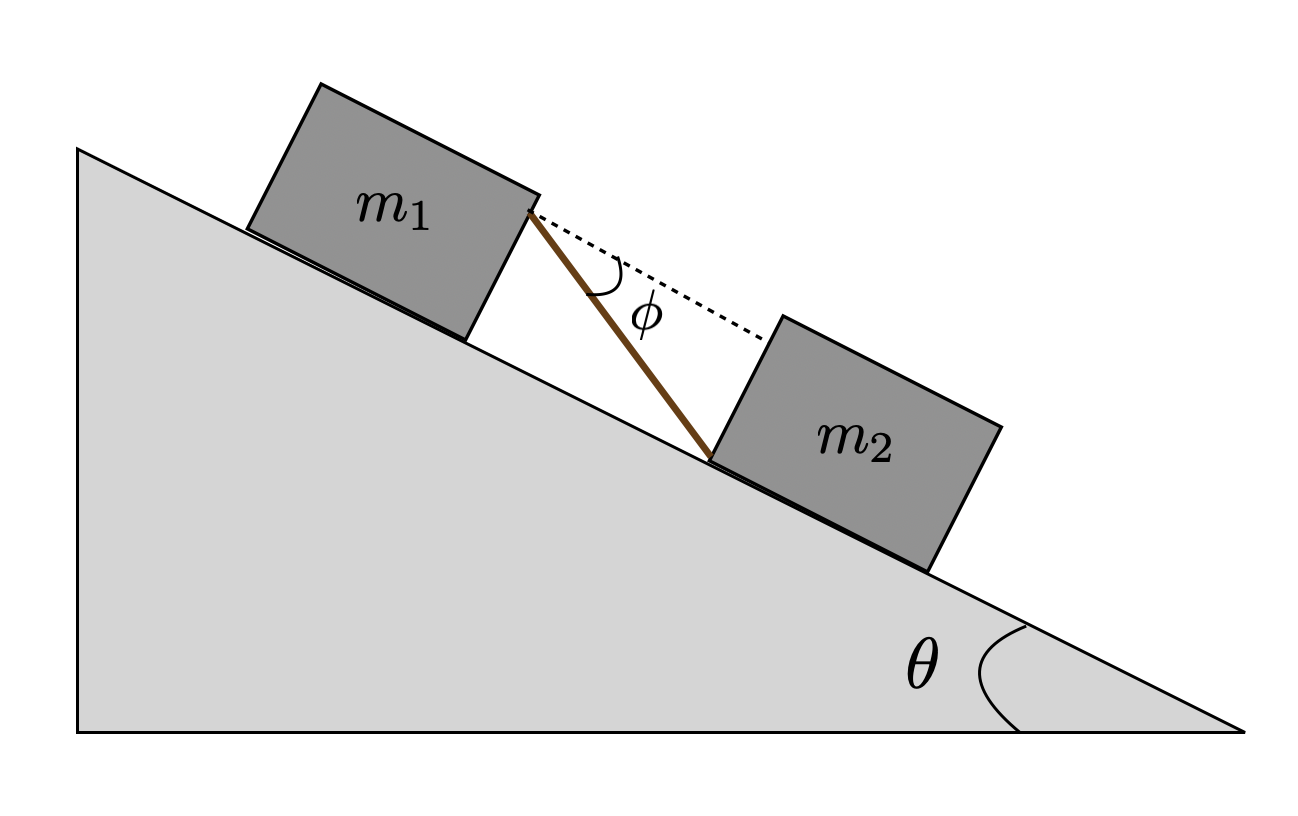
\includegraphics[scale=0.5]{m1m2}
\caption{Figure for problem 3.}\label{fig1}
\end{figure}
\section*{Problem 4}
A large mass $M$ hangs (stationary) at the end of a string that passes through a smooth tube to a small mass $m$ that whirls around in a circular path of radius $l\sin\theta$, where $l$ is the length of the string $m$ to the top end of the tube (see Fig. \ref{fig2}). Write down the dynamical equations that apply to each mass and show that $m$ must complete one orbit in a time of $2\pi(lm/gM)^{1/2}$. Consider whether there is any restriction on the value of the angle $\theta$ in this motion.
\begin{figure}
\center
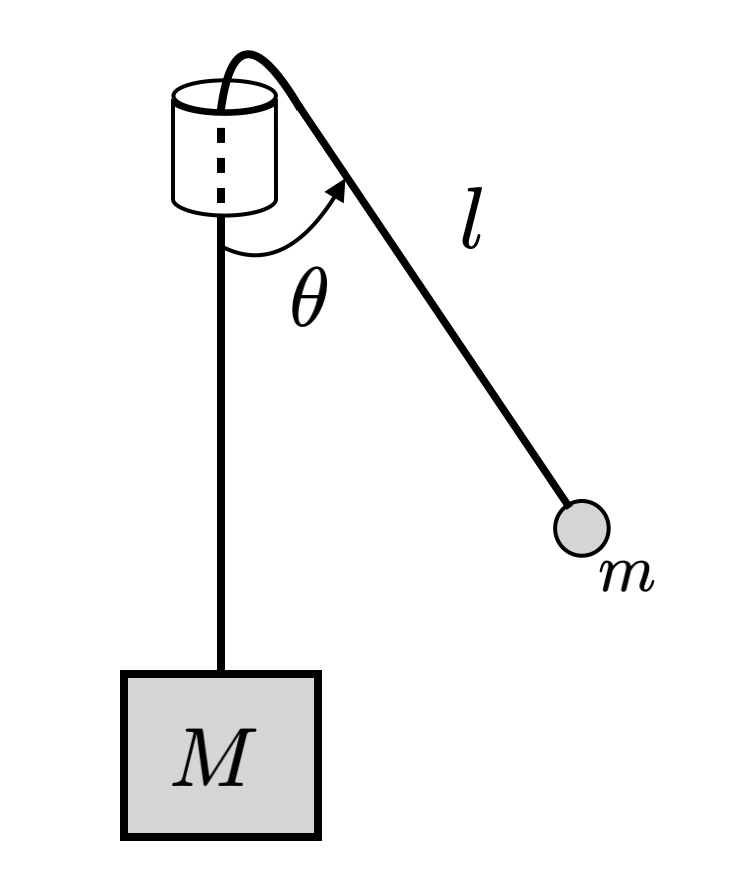
\includegraphics[scale=0.5]{rotate}
\caption{Figure for problem 4.}\label{fig2}
\end{figure}
\section*{Problem 5}
The speed of a body released from rest falling through viscous medium (for instance, an iron pellet falling in a jar full of oil) is given by the formula 
\begin{align}
v=-g\tau+g\tau e^{-t/\tau}
\end{align}
where $\tau$ is a constant that depends on the size and shape of the body and on the viscosity of the medium and $e=2.718\cdots$ is the basis of the natural logarithms.
\begin{enumerate}[label=(\roman*)]
\item Find the acceleration as a function of time.
\item Show that for $t\rightarrow\infty$, the speed approaches terminal value $-g\tau$.
\item By differentiation, verify that the equation for the position as a function of time consistent with the above expression for the speed is 
\begin{align}
x=-g\tau t-g\tau^{2}e^{-t/\tau}+g\tau^{2}+x_{0}
\end{align}
\item Show that for small vales of $t$ ($t\ll\tau$), the equation for $x$ is approximately $x\approx \dfrac{-1}{2}gt^{2}+x_{0}$.
\end{enumerate}




\end{document}



